\documentclass{article}

% if you need to pass options to natbib, use, e.g.:
% \PassOptionsToPackage{numbers, compress}{natbib}
% before loading nips
%
% to avoid loading the natbib package, add option nonatbib:
% \usepackage[nonatbib]{nips_2017}

%\usepackage{nips}

% to compile a camera-ready version, add the [final] option, e.g.:
\usepackage[final]{nips}
\usepackage[linesnumbered,boxed,ruled,commentsnumbered]{algorithm2e}
\usepackage{amsmath}
\usepackage[linesnumbered,boxed]{algorithm2e}
\usepackage[utf8]{inputenc} % allow utf-8 input
\usepackage[T1]{fontenc}    % use 8-bit T1 fonts
\usepackage{hyperref}       % hyperlinks
\usepackage{url}            % simple URL typesetting
\usepackage{booktabs}       % professional-quality tables
\usepackage{amsfonts}       % blackboard math symbols
\usepackage{nicefrac}       % compact symbols for 1/2, etc.
\usepackage{microtype}      % microtypography
\usepackage[linesnumbered,boxed,ruled,commentsnumbered]{algorithm2e}
\usepackage{listings}
\usepackage{multirow}
\usepackage{graphicx}
\usepackage[justification=centering]{caption}

\title{Large-scale Optimal Transport}

% The \author macro works with any number of authors. There are two
% commands used to separate the names and addresses of multiple
% authors: \And and \AND.
%
% Using \And between authors leaves it to LaTeX to determine where to
% break the lines. Using \AND forces a line break at that point. So,
% if LaTeX puts 3 of 4 authors names on the first line, and the last
% on the second line, try using \AND instead of \And before the third
% author name.


\author{
  Weijie Chen\thanks{Pre-admission 2019 PKU AAIS} \\
  School of Physics\\
  Peking University\\
  1500011335 \\
  \texttt{1500011335@pku.edu.cn} \\
  \And
  Dinghuai Zhang \\
  School of Mathematics\\
  Peking University\\
  1600013525\\
  \texttt{1600013525@pku.edu.cn} \\
}



\begin{document}
% \nipsfinalcopy is no longer used

\maketitle

\begin{abstract}
  
\end{abstract}

\section{Introduction to Optimal Transport}

\section{Problem Statement}
The standard formulation of optimal transport are derived from couplings. [\textbf{Villani2009}] That is, let $ \left(\mathcal{X}, \mu \right)$ and $\left(\mathcal{Y}, \nu \right)$  be two probability spaces, and a probability distribution $\pi$ on $ \mathcal{X} \times \mathcal{Y} $ is called \emph{coupling} if $ proj_{\mathcal{X}} (\pi) = \mu $ and $ proj_{\mathcal{Y}} (\pi)= \nu $. An optimal transport between $ \left(\mathcal{X}, \mu \right)  $ and $ \left(\mathcal{Y}, \nu \right) $, or an optimal coupling, is a coupling minimize
\begin{equation}
\int_{ \mathcal{X} \times \mathcal{Y} } c ( x, y)  d \pi ( x, y ) 
\end{equation}

Optimal transport problems can be categorized according to the discreteness of $\mu$ and $\nu$. In this report, we only consider discrete optimal tranport problems, where the two distributions are distributions of finite weighted points.

A discrete optimal transport problem can be formulated into a linear program as
\begin{equation} \label{Eq:StdLP}
\begin{aligned}
\min_{\pi} & \sum_{i=1}^{m}\sum_{j=1}^{n} c_{ i j } \pi_{ i j }\\
s.t. & \sum_{j=1}^{n}\pi_{ i j } = \mu_i, \forall i\\
& \sum_{i=1}^{m}\pi_{ i j } = \nu_j, \forall j \\
& \pi_{ij} \geq 0,
\end{aligned}
\end{equation}
where $c$ stands for the cost and $s$ for the transportation plan, while $\mu$ and $\nu$ are restrictions. Note that we always suppose $ c \geq 0 $, $ \mu \geq 0 $, $ \nu \geq 0 $ and $ \sum_{i=1}^{m}{\mu_i} = \sum_{j=1}^{n}{\nu_j} = 1 $ implicitly. From realistic background, $c$ is always valued the squared Euclidean distanced or some other norms. Note that there are $ m n $ variables in this formulation, and this leads to intensive computation.

In order to decrease the number of variables, we can derive the dual problem of discrete optimal transport.
\begin{equation} \label{Eq:StdLP_dual}
  \begin{aligned}
  \max_{\lambda,\eta} & \sum_{i=1}^{m}\mu_{i}\lambda_{i}+\sum_{j=1}^{n}\nu_{j}\eta_{j}\\
  s.t. & c_{i j}-\lambda_{i}-\eta_{j}\geq0, \forall i, j
  \end{aligned}
\end{equation}
Although this formulation only has m + n variables, there are still challenges including the recovery of $\pi$ from $\lambda$ and $\eta$ and the great number of constraints.
\section{Algorithms}
\subsection{ADMM for Primal Problem}
We first implement a first order algorithm called \textbf{alternative direction method of multipliers} (ADMM). According to a reformulation of primal problem, 
\begin{equation} \label{Eq:StdLP_admm_primal}
  \begin{aligned}
  \min_{\pi} & \sum_{i=1}^{m}\sum_{j=1}^{n} c_{ i j } \pi_{ i j }+\mathbb{I}_{+}(\hat{\pi})\\
  s.t. & \sum_{j=1}^{n}\pi_{ i j } = \mu_i, \forall i\\
  & \sum_{i=1}^{m}\pi_{ i j } = \nu_j, \forall j \\
  & \pi=\hat{\pi}
  \end{aligned}
\end{equation}
where $\mathbb{I}_{+}$ is indicator of $\mathbb{R}^{m\times n}_{+}$. The augmented Lagrangian can be written as 
\begin{equation} \label{Eq:admm_primal}
  \begin{aligned}
\mathcal{L}_{\rho}(\pi,\hat{\pi},\lambda,\eta,e)=&\sum_{i=1}^{m}\sum_{j=1}^{n} c_{ i j } \pi_{ i j }+\mathbb{I}_{+}(\hat{\pi})\\
&+\sum_{i=1}^{m}\lambda_{i}\left(\mu_i-\sum_{j=1}^{n}\pi_{ i j }\right)+\sum_{j=1}^{n}\eta_{j}\left(\nu_j-\sum_{i=1}^{m}\pi_{ i j }\right)+\sum_{i=1}^{m}\sum_{j=1}^{n}e_{ij}\left(\pi_{ij}-\hat{\pi}_{ij}\right)\\
&+\frac{\rho}{2}\sum_{i=1}^{m}\left(\mu_i-\sum_{j=1}^{n}\pi_{ i j }\right)^{2}+\frac{\rho}{2}\sum_{j=1}^{n}\left(\nu_j-\sum_{i=1}^{m}\pi_{ i j }\right)^{2}+\frac{\rho}{2}\sum_{i=1}^{m}\sum_{j=1}^{n}\left(\pi_{ij}-\hat{\pi}_{ij}\right)^{2}
\end{aligned}
\end{equation}
The minimizer of $\hat{\pi}$ can be written easily as
\begin{equation}
  argmin_{\hat{\pi}}\mathcal{L}_{\rho}(\pi,\hat{\pi},\lambda,\eta,e)=max\left(\pi+\frac{e}{\rho}, 0\right)
\end{equation}

For the minimizer of $\pi$, we can derive the following equation:
\begin{equation}
  \sum _ { k = 1 } ^ { n } \pi _ { i k } + \sum _ { k = 1 } ^ { m } \pi _ { k j } + \pi_ { i j } = \frac { 1 } { \rho } \left(-e _ { i j } + \lambda _ { i } + \eta _ { j } - c _ { i j } \right) + \mu _ { i } + v _ { j } + \hat{ \pi} _ { i j } \equiv r _ { i j }
\end{equation}
It's a linear equation of $\pi_{ij}$ for the given $r_{ij}$,  which can be solved directly.
\begin{equation}
\pi_ { i j } = r _ { i j } - \frac { 1 } { n + 1 } \sum _ { k = 1 } ^ { n } \left( r _ { i k } - \frac { 1 } { m + n + 1 } \sum _ { l = 1 } ^ { m } r _ { l k } \right) - \frac { 1 } { m + 1 } \sum _ { k = 1 } ^ { m } \left( r _ { k j } - \frac { 1 } { m + n + 1 } \sum _ { l = 1 } ^ { n } r _ { k l } \right)
\end{equation}

Then, we can write the explicit form of ADMM algorithm. This algorithm is implemented in \textbf{ADMM$\_$primal.py}.

\begin{algorithm}[H]
  \SetAlgoNoLine
  \caption{Alternating direction method of multipliers for the primal problem} 
  \KwIn{input data $c$, $\mu$, $\nu$, 
  step size$\alpha$, penalty scalar $\rho$ and maximum iteration $N$} 
  \KwOut{solution $\pi$} 
  initializing $k = 0$\\
  $\pi^{(k)},\hat{\pi}^{(k)},e^{(k)},\lambda^{(k)},\eta^{(k)}:=0$\\
  \While{ $k<N$} 
  {  
   $\pi^{(k+1)}:=argmin_{\pi}\mathcal{L}_{\rho}(\pi,\hat{\pi}^{(k)},\lambda^{(k)},\eta^{(k)},e^{(k)})$\\
   $\hat{\pi}^{(k+1)}:=argmin_{\hat{\pi}}\mathcal{L}_{\rho}(\pi^{(k+1)},\hat{\pi},\lambda^{(k)},\eta^{(k)},e^{(k)})$\\
   $\lambda^{(k+1)}:=\lambda^{(k)}+\alpha\rho(\mu-\sum_{j=1}^{n}\pi_{ i j })$\\
   $\eta^{(k+1)}:=\eta^{(k)}+\alpha\rho(\nu-\sum_{i=1}^{m}\pi_{ i j })$\\
   $e^{(k+1)}:=e^{(k)}+\alpha\rho(\pi-\hat{\pi})$\\
   $k:= k+1$
  }
  return $\hat{\pi}$
\end{algorithm}

\subsection{ADMM for Dual Problem}
According the reformulation of dual problem,
\begin{equation}
  \begin{aligned}
    \min_{\lambda,\eta} & -\sum_{i=1}^{m}\mu_{i}\lambda_{i}-\sum_{j=1}^{n}\nu_{j}\eta_{j}+\mathbb{I}_{+}(e)\\
    s.t. & c_{i j}-\lambda_{i}-\eta_{j}-e_{ij}=0, \forall i, j
    \end{aligned}
\end{equation} 
we can write down the augmented Lagrangian as
\begin{equation} \label{Eq:admm_dual}
  \begin{aligned}
\mathcal{L}_{\rho}(\lambda,\eta,e,d)=&-\sum_{i=1}^{m}\mu_{i}\lambda_{i}-\sum_{j=1}^{n}\nu_{j}\eta_{j}+\mathbb{I}_{+}(e)\\
&+\sum_{i=1}^{m}\sum_{j=1}^{n}d_{ij}(c_{i j}-\lambda_{i}-\eta_{j}-e_{ij})+\frac{\rho}{2}\sum_{i=1}^{m}\sum_{j=1}^{n}(c_{i j}-\lambda_{i}-\eta_{j}-e_{ij})^{2}
\end{aligned}
\end{equation}
The minimizer of $e$ can be done directly by solving for zero gradient and projection, while
the minimizer of $\lambda$ and $\eta$ can be done by solving for zero gradient.
\begin{equation}
  \begin{aligned}
    argmin_{e_{ij}}\mathcal{L}_{\rho}(\lambda,\eta,e,d)=& max\left(c_{ij}+\frac{d_{ij}}{\rho}-\lambda_{i}-\eta_{j}, 0\right)\\
    argmin_{\lambda_{i}}\mathcal{L}_{\rho}(\lambda,\eta,e,d)=& \frac{1}{n}\left((\mu_{i}+\sum_{j=1}^{n}d_{ij})/\rho+\sum_{j=1}^{n}(c_{ij}-\eta_{j}-e_{ij})\right)\\
    argmin_{\eta_{j}}\mathcal{L}_{\rho}(\lambda,\eta,e,d)=& \frac{1}{m}\left((\nu_{j}+\sum_{i=1}^{m}d_{ij})/\rho+\sum_{i=1}^{m}(c_{ij}-\lambda_{i}-e_{ij})\right)\\
  \end{aligned}
\end{equation}

The algorithm is implemented in \textbf{ADMM$\_$dual.py}.
Solution $\pi$ can be recovered by $\pi=-d$ from KKT conditions.

\begin{algorithm}[H]
  \SetAlgoNoLine
  \caption{Alternating direction method of multipliers for the primal problem} 
  \KwIn{input data $c$, $\mu$, $\nu$, 
  step size$\alpha$, penalty scalar $\rho$ and maximum iteration $N$} 
  \KwOut{solution $\pi$} 
  initializing $k = 0$\\
  $\lambda^{(k)},\eta^{(k)},e^{(k)},d^{(k)}:=0$\\
  \While{ $k<N$} 
  {  
   $\lambda^{(k+1)}_{i}:=argmin_{\lambda_{i}}\mathcal{L}_{\rho}(\lambda,\eta^{(k)},e^{(k)},d^{(k)})$\\
   $\eta^{(k+1)}_{j}:=argmin_{\eta_{j}}\mathcal{L}_{\rho}(\lambda^{(k+1)},\eta,e^{(k)},d^{(k)})$\\
   $e^{(k+1)}_{ij}:=argmin_{e_{ij}}\mathcal{L}_{\rho}(\lambda^{(k+1)},\eta^{(k+1)},e,d^{(k)})$\\
   $d^{(k+1)}_{ij}:=d^{(k)}_{ij}+\alpha\rho(c_{ij}-\lambda_{i}-\eta_{j}-e_{ij})$\\
   $k:= k+1$
  }
  return $\pi=-d$
\end{algorithm}
\subsection{Add Entropy Regularization: Sinkhorn-Knopp Method }
The discrete entropy of a coupling matrix is defined as
\begin{equation}
\mathbf { H } ( \mathbf { P } ) \stackrel { \mathrm { def } } { = } - \sum _ { i , j } \mathbf { P } _ { i , j } \left( \log \left( \mathbf { P } _ { i , j } \right) - 1 \right)
\end{equation}
The function $\mathbf{H}$ is strongly concave.

The idea of the entropic regularization of optimal transport is to use $-\mathbf{H}$ as a regularizing function to obtain approximate solutions to the original transport problem:
\begin{equation}
\mathrm { L } _ { \mathrm { C } } ^ { \varepsilon } ( \mathbf { a } , \mathbf { b } ) \stackrel { \mathrm { def } } { = } \min _ { \mathbf { P } \in \mathbf { U } ( \mathbf { a } , \mathbf { b } ) } \langle \mathbf { P } , \mathbf { C } \rangle - \varepsilon \mathbf { H } ( \mathbf { P } )
\label{sinkhorn target}
\end{equation}
(Actually, this can be interpreted as $\text{KL}(\mathbf{P}||\mathbf{K})$)

One can show that the solution to \ref{sinkhorn target} has the form of 
\begin{equation}
\mathbf { P } _ { i , j } = \mathbf { u } _ { i } \mathbf { K } _ { i , j } \mathbf { v } _ { j }
\end{equation}
where $\mathbf { K } _ { i , j } = e^{-\mathbf{C}_{i,j}/\epsilon}$ by calculating the KKT condition:
Introducing two dual variables $\mathbf { f } \in \mathbb { R } ^ { n } , \mathbf { g } \in \mathbb { R } ^ { n }$ and calculate the lagrangian:
\begin{equation}
\mathcal { L } ( \mathbf { P } , \mathbf { f } , \mathbf { g } ) = \langle \mathbf { P } , \mathbf { C } \rangle - \varepsilon \mathbf { H } ( \mathbf { P } ) - \left\langle \mathbf { f } , \mathbf { P } \mathbf { 1 } _ { n } - \mathbf { a } \right\rangle - \left\langle \mathbf { g } , \mathbf { P } ^ { \mathrm { T } } \mathbf{ 1 } _ { n } - \mathbf { b } \right\rangle
\end{equation}
take first order gradient and we get
\begin{align}
\frac { \partial \mathcal { L } ( \mathbf { P } , \mathbf { f } , \mathbf { g } ) } { \partial \mathbf { P } _ { i , j } } &= \mathbf { C } _ { i , j } + \varepsilon \log \left( \mathbf { P } _ { i , j } \right) - \mathbf { f } _ { i } - \mathbf { g } _ { j } = 0\\
\Rightarrow\mathbf { P } _ { i , j } &= e ^ { \mathbf { f } _ { i } / \varepsilon } e ^ { - \mathbf { C } _ { i , j } / \varepsilon } e ^ { \mathbf { g } _ { j } / \varepsilon }
\label{solution for P}
\end{align}
Based on the constrain that:
\begin{align}
\operatorname { diag } ( \mathbf { u } ) \mathbf { K } \operatorname { diag } ( \mathbf { v } ) \mathbf { 1 } _ { m } &= \mathbf { a }\\
\operatorname { diag } ( \mathbf { v } ) \mathbf { K } ^ { \top } \operatorname { diag } ( \mathbf { u } ) \mathbf { 1 } _ { n } &= \mathbf { b }
\end{align}
or :
\begin{align}
\mathbf { u } \odot ( \mathbf { K } \mathbf { v } ) = \mathbf { a } \quad \text { and } \quad \mathbf { v } \odot \left( \mathbf { K } ^ { \mathrm { T } } \mathbf { u } \right) = \mathbf { b }
\label{solution for marginal}
\end{align}
(where $\odot$ means entry-wise multiplication of vectors) we can develop our algorithm as iteratively updating $\mathbf { u }$ and $\mathbf { v }$:
\begin{align}
\mathbf { u } ^ { ( \ell + 1 ) }  { = } \frac { \mathbf { a } } { \mathbf { K } \mathbf { v } ^ { ( \ell ) } } \text { and } \mathbf { v } ^ { ( \ell + 1 ) } { = } \frac { \mathbf { b } } { \mathbf { K } ^ { \mathrm { T } } \mathbf { u } ^ { ( \ell + 1 ) } }
\end{align}
with $\mathbf { v } ^ { ( 0 ) } = \mathbf { 1 } _ { m }$ and $\mathbf { K } _ { i , j } = e^{-\mathbf{C}_{i,j}/\epsilon}$.

\subsection{Sinkhorn-Newton Method}
From \ref{solution for P} and \ref{solution for marginal} we can conclude that our target could be reformulated as finding a zero point of

\begin{displaymath}
F(\mathbf { f },\mathbf { g}) :=
\left( \begin{array}{c}
a -  \operatorname { diag } (   e ^ { -\mathbf { f }  / \epsilon } ) \mathbf { K }  e ^ { -\mathbf { g }  / \epsilon } \\
b -  \operatorname { diag } (   e ^ { -\mathbf { g }  / \epsilon } ) \mathbf { K }  e ^ { -\mathbf { f }  / \epsilon }
\end{array} \right)
\end{displaymath}
where $a,b,\epsilon$ and $\mathbf { K}$ are known.
What we need to do is to use newton-raphson method to find its zero points:
\begin{align}
\left( \begin{array} { l } { \mathbf { f }^ { k + 1 } } \\ { \mathbf { g } ^ { k + 1 } } \end{array} \right) = \left( \begin{array} { l } { \mathbf { f } ^ { k } } \\ { \mathbf { g } ^ { k } } \end{array} \right) - J _ { F } \left( \mathbf { f } ^ { k } , \mathbf { g } ^ { k } \right) ^ { - 1 } F \left( \mathbf { f } ^ { k } , \mathbf { g } ^ { k } \right)
\end{align}
where the Jacobian of F is:
\begin{align}
J _ { F } ( \mathbf { f }  ,  \mathbf { g } ) = \frac { 1 } { \varepsilon } \left[ \begin{array} { c c } { \operatorname { Diag } \left( \mathbf{P} \mathbf { 1 } _ { m } \right) } & { \mathbf{P} } \\ { \mathbf{P} ^ { \top } } & { \operatorname { Diag } \left( \mathbf{P} ^ { \top } \mathbf { 1 } _ { n } \right) } \end{array} \right]
\end{align}
that is, we can use conjugate gradient to solve
\begin{align}
J _ { F } \left(  \mathbf {f} ^ { k } ,  \mathbf {g} ^ { k } \right) \left( \begin{array} { c } { \delta  \mathbf {f} } \\ { \delta  \mathbf {g} } \end{array} \right) = - F \left(  \mathbf {f} ^ { k } ,  \mathbf {g} ^ { k } \right)
\end{align}
and then update variables by
\begin{align}
\begin{aligned}  \mathbf {f} ^ { k + 1 } & =  \mathbf {f} ^ { k } + \delta  \mathbf {f} \\  \mathbf {g} ^ { k + 1 } & =  \mathbf {g} ^ { k } + \delta  \mathbf {g} \end{aligned}
\end{align}
Because $ \mathbf {P} ^ { k } : = \operatorname { Diag } \left( \mathrm { e } ^ { -  \mathbf {f} ^ { k } / \varepsilon } \right) \mathbf { K} \operatorname { Diag } \left( \mathrm { e } ^ { -  \mathbf {g} ^ { k } / \varepsilon } \right)$, the update step can be rewrite as
\begin{align}
\begin{aligned}  \mathbf {P} ^ { k + 1 } & = \operatorname { Diag } \left( \mathrm { e } ^ { - \left[  \mathbf {f} ^ { k } + \delta  \mathbf {f} \right] / \varepsilon } \right)  \mathbf {K} \operatorname { Diag } \left( \mathrm { e } ^ { - \left[  \mathbf {g} ^ { k } + \delta  \mathbf {g} \right] / \varepsilon } \right) \\ & = \operatorname { Diag } \left( \mathrm { e } ^ { - \delta  \mathbf {f} / \varepsilon } \right)  \mathbf {P} ^ { k } \operatorname { Diag } \left( \mathrm { e } ^ { - \delta  \mathbf {g} / \varepsilon } \right) \end{aligned}
\end{align}


\begin{algorithm}[H]
  \SetAlgoNoLine
  \caption{Sinkhorn-Newton method in primal variable} 
  \KwIn{$\mathbf{a} \in \Sigma _ { n } , \mathbf{b} \in \Sigma _ { m } , \mathbf{C} \in \mathbb { R } ^ { n \times m }$} 
   initializing $\mathbf{P} ^ { 0 } = \exp ( - \mathbf{C} / \varepsilon ) ,$ set $k = 0$\\
  \Repeat
  { some stopping criteria fulfilled }{
 $\mathbf{a} ^ { k } \gets \mathbf{P} ^ { k } \mathbf{1}_ { m }$\\  
 $\mathbf{b} ^ { k } \gets \left( \mathbf{P} ^ { k } \right) ^ { \top } \mathbf { 1 } _ { n }$\\
  compute $\delta \mathbf{f}, \delta \mathbf{g}$: 
  \quad$\frac { 1 } { \varepsilon } \left[ \begin{array} { c c } { \operatorname { Diag } \left( \mathbf{a} ^ { k } \right) } & { \mathbf{P} ^ { k } } \\ { \left( \mathbf{P} ^ { k } \right) ^ { \top } } & { \operatorname { Diag } \left( \mathbf{b} ^ { k } \right) } \end{array} \right] \left[ \begin{array} { l } { \delta \mathbf{f} } \\ { \delta \mathbf{g} } \end{array} \right] = \left[ \begin{array} { l } { \mathbf{a} ^ { k } - \mathbf{a} } \\ { \mathbf{b} ^ { k } - \mathbf{b} } \end{array} \right]$\\
$\mathbf{P} ^ { k + 1 } \gets \operatorname { Diag } \left( \mathrm { e } ^ { - \delta \mathbf{f} / \varepsilon } \right) \mathbf{P} ^ { k } \operatorname { Diag } \left( \mathrm { e } ^ { - \delta \mathbf{g} / \varepsilon } \right)$\\
   $k\gets k+1$
  }
  return $\mathbf{P}$
\end{algorithm}

\subsection{Sinkhorn-Newton for Dual Method}

\begin{algorithm}[H]
  \SetAlgoNoLine
  \caption{Sinkhorn-Newton method in dual variable} 
  \KwIn{$\mathbf{a} \in \Sigma _ { n } , \mathbf{b} \in \Sigma _ { m } , \mathbf{K} \ and\ \mathbf{K} ^ { \top }$} 
  \KwOut{solution $\mathbf{P}$} 
  initializing $a ^ { 0 } \in \mathbb { R } ^ { n } , b ^ { 0 } \in \mathbb { R } ^ { m } , \operatorname { set } k = 0$\\
  \Repeat
  { some stopping criteria fulfilled }{
 $a ^ { k }\gets  \mathrm { e } ^ { - f ^ { k } / \varepsilon } \odot K \mathrm { e } ^ { - g ^ { k } / \varepsilon }$\\
 $b ^ { k } \gets  \mathrm { e } ^ { - g ^ { k } / \varepsilon } \odot K ^ { \top } \mathrm { e } ^ { - f ^ { k } / \varepsilon }$\\
 Compute updates $\delta f$ and $\delta g$ by solving
$M \left[ \begin{array} { c } { \delta f } \\ { \delta g } \end{array} \right] = \left[ \begin{array} { c } { a ^ { k } - a } \\ { b ^ { k } - b } \end{array} \right]$\\
   where the application of $M$ is given by
$M \left[ \begin{array} { c } { \delta f } \\ { \delta g } \end{array} \right] = \frac { 1 } { \varepsilon } \left[ \begin{array} { c } { a ^ { k } \odot \delta f + \mathrm { e } ^ { - f ^ { k } / \varepsilon } \odot K \left( \mathrm { e } ^ { - g ^ { k } / \varepsilon } \odot \delta g \right) } \\ { b ^ { k } \odot \delta g + e ^ { - g ^ { k } / \varepsilon } \odot K ^ { \top } \left( \mathrm { e } ^ { - f ^ { k } / \varepsilon } \odot \delta f \right) } \end{array} \right]$\\
$f ^ { k + 1 } \gets f ^ { k } + \delta f$\\
$g ^ { k + 1 } \gets  g ^ { k } + \delta g$\\
$k\gets k+1$
  }
  return $\mathbf{P}$
\end{algorithm}


\section{Numerical Result and Interpretation}
\subsection{Description of datasets}
In order to compare the performance of differnet algorithms, we have to use some classic and challenging datasets.

In general, the $i$-th datapoint can be denoted as $(x_{i},\mu_{i})$ , where $x_{i}\in \mathbb{R}^{d}$ is the position of datapoint and $\mu_{i}$ is the probability at $x_{i}$.

For convenience, we assume that datapoints are followed 2D distribution (i.e. $x_{i}\in \mathbb{R}^{2}$ ). Besides, we use the squared Euclidean distance to define the cost matrix between two datasets $\{(x_{i},\mu_{i})\}_{i=1}^{m}$ and $\{(y_{j},\nu_{j})\}_{j=1}^{n}$ as following
\begin{equation}
  c_{ij}=||x_{i}-y_{j}||_{2}^{2}\quad\forall i, j
\end{equation}
We have tested our algorithms on four types of datasets
\begin{itemize}
  \item Randomly generated dataset\\
        The position are uniformly sampled from
        $[0, 1]\times[0, 1]$. The weights $\mu$ and $\nu$ are randomly sampled from $[0, 1]$ and scaled to $ \sum_{i=1}^{m}{\mu_i} = \sum_{j=1}^{n}{\nu_j} = 1 $.
  \item ellipses [\textbf{Gerber2017}]\\
  The ellipse example consists of two uniform samples (source and target data set) of size $m=n$ from the unit circle
  with normal distributed noise added with zero mean and standard deviation 0.1. The source
  data sample is then scaled in the x-Axis by 0.5 and in the y-Axis by 2, while the target
  data set is scaled in the x-Axis by 2 and in the y-Axis by 0.5.
  Besides, the weights are both normalized uniform distributions.
  \item Caffarelli [\textbf{Gerber2017}]\\
  Caffarelli’s example consists of two uniform samples (source and target data set) on $[-1, 1]\times[-1, 1]$  of size $m=n$. Any points outside the unit circle are then
discarded. Additionally, the target data sample is split along the x-Axis at 0 and shifted by
$+2$ and $-2$ for points with positive and negative x-Axis values, respectively. The weights are both normalized uniform distributions, too.
  \item DOTmark [\textbf{Schrieber2017}]\\
  In DOTmark, we always have $m=n=r^{2}$, and $(x_i)_{1\leq i\leq m} = (y_j)_{1\leq j\leq n}$ form a regular square grid of resolution $r\times r$ in $\mathbb{R}^{2}$, which are the natural position of source and target data set. The weights are the brightness distributions with normalization. Besides, DOTmark consists of 10 classes of 10 different
  images, each of which is available at the 5 different
  resolutions from $32\times32$ to $512\times512$ (in doubling steps per dimension).
\end{itemize}
\begin{figure}[h]
  \centering
  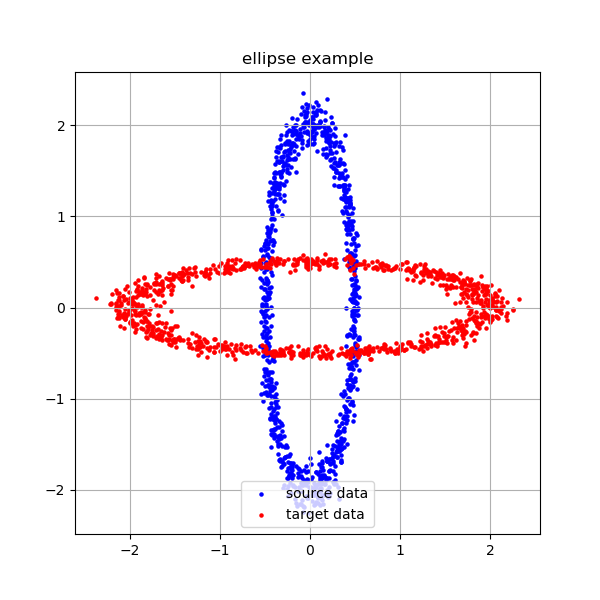
\includegraphics[width=.5\textwidth]{ellip.png}
  \captionsetup{justification=centering}
  \caption{\label{fig:ellip}$m=n=1000$, ellipse example}
\end{figure}
\begin{figure}[h]
  \centering
  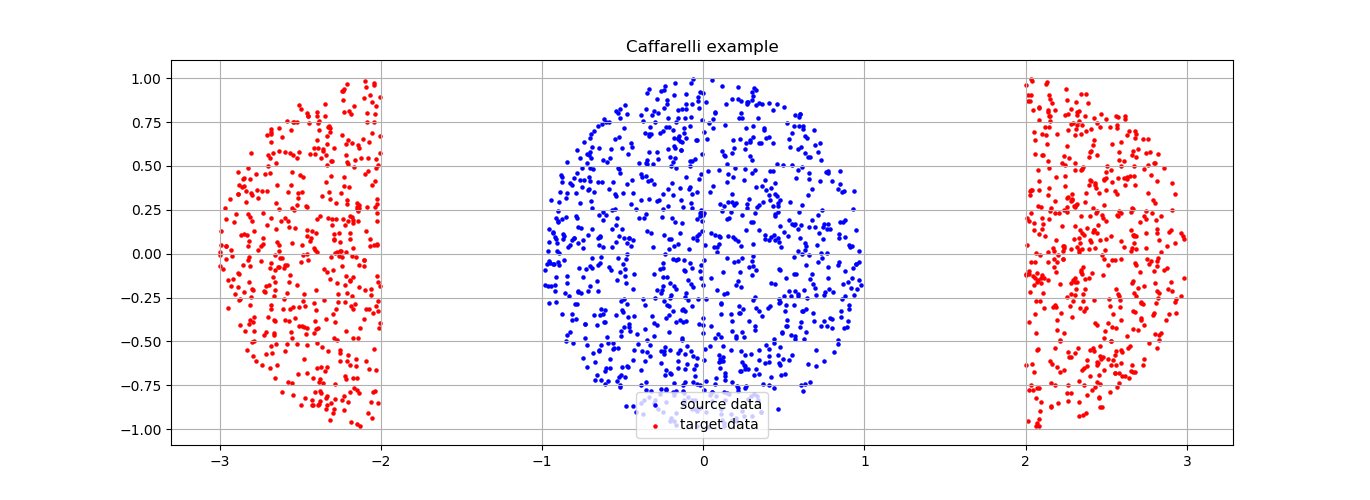
\includegraphics[width=.9\textwidth]{caffa.png}
  \captionsetup{justification=centering}
  \caption{\label{fig:caffa}$m=n=1000$, Caffarelli’s example}
\end{figure}
\begin{table}[h]
  \centering
  \begin{tabular}{|c|c|}
  \hline
  $\#$&Name\\
  \hline
  \hline
  1&WhiteNoise\\
  2&GRFrough\\
  3&GRFmoderate\\
  4&GRFsmooth\\
  5&LogGRF\\
  6&LogitGRF\\
  7&CauchyDensity\\
  8&Shapes\\
  9&ClassicImages\\
  10&Microscopy\\
  \hline
  \end{tabular}
  \caption{\label{tab:table1}The 10 classes in the DOTmark}
\end{table}
\subsection{Numerical result}
\begin{table}[h]
  \centering
  \begin{tabular}{|c|c|cccccc|}
    \hline
    $m=n$&&M primal&M dual&M int&G primal&G dual&G int\\
    \hline
    \hline
  \multirow{4}*{256}&dist&5.45e-3&7.25e-3&8.09e-3&5.94e-3&8.62e-3&5.13e-3\\
  ~&time&3.43e-1&3.75e-1&5.28e-1&6.79e-1&7.07e-1&8.56e-1\\  
  ~&err $\mu$&1.79e-5&2.04e-17&2.31e-12&1.34e-17&9.97e-18&4.34e-18\\   
  ~&err $\nu$&1.79e-5&2.45e-16&2.79e-12&5.36e-16&3.87e-16&5.05e-16\\
  \hline
  \multirow{4}*{512}&dist&2.90e-3&2.88e-3&3.37e-3&3.79e-3&2.91e-3&5.52e-3\\
  ~&time&1.39&1.70&2.93&2.83&3.40&4.27\\  
  ~&err $\mu$&4.35e-5&2.67e-17&1.30e-13&1.08e-17&1.09e-15&1.21e-17\\   
  ~&err $\nu$&4.35e-5&1.09e-16&1.04e-13&1.72e-16&1.26e-17&7.46e-16\\
  \hline
  \multirow{4}*{1024}&dist&1.78e-3&1.94e-3&1.89e-3&1.91e-3&1.80e-3&1.84e-3\\
  ~&time&8.11&15.3&15.2&14.1&14.0&18.7\\  
  ~&err $\mu$&1.04e-4&1.09e-16&1.38e-12&1.01e-17&1.12e-17&1.91e-15\\   
  ~&err $\nu$&1.04e-4&1.91e-15&1.27e-12&6.49e-16&3.42e-16&9.43e-18\\
  \hline
  \multirow{4}*{2048}&dist&1.35e-3&1.36e-3&1.31e-3&1.42e-3&1.46e-3&1.49e-3\\
  ~&time&35.0&1.05e+2&68.7&3.45e+2&58.4&88.9\\  
  ~&err $\mu$&2.71e-4&2.61e-16&1.81e-12&9.41e-18&6.09e-16&4.95e-16\\   
  ~&err $\nu$&2.7e-4&1.79e-15&2.27e-12&1.27e-15&1.17e-17&1.13e-17\\
  \hline
  \end{tabular}
  \caption{\label{tab:table1}random}
\end{table}
\begin{table}[h]
  \centering
  \begin{tabular}{|c|c|cccccc|}
    \hline
    $m=n$&&M primal&M dual&M int&G primal&G dual&G int\\
    \hline
    \hline
  \multirow{4}*{256}&dist&2.37&2.27&1.88&2.28&2.12&2.26\\
  ~&time&5.42e-1&9.80&4.10&6.57e-1&1.49&7.22e-1\\  
  ~&err $\mu$&1.76e-5&9.54e-18&1.65e-12&0&0&0\\   
  ~&err $\nu$&1.76e-5&9.54e-18&1.65e-12&0&0&0\\
  \hline
  \multirow{4}*{512}&dist&2.36&2.39&2.24&2.15&2.31&2.32\\
  ~&time&1.65&5.01&1.49&4.87&4.62&4.01\\  
  ~&err $\mu$&4.05e-5&2.04e-17&2.01e-11&0&0&0\\   
  ~&err $\nu$&4.05e-5&1.95e-17&2.01e-11&0&0&0\\
  \hline
  \multirow{4}*{1024}&dist&2.24&2.11&2.21&2.24&2.18&2.27\\
  ~&time&7.89&70.4&9.73&64.5&21.9&16.6\\  
  ~&err $\mu$&9.39e-5&1.59e-16&5.37e-10&0&0\\   
  ~&err $\nu$&9.39e-5&1.48e-16&5.37e-10&0&0\\
  \hline
  \multirow{4}*{2048}&dist&2.38&2.23&2.28&2.27&2.22&2.37\\
  ~&time&32.6&4.37e+2&47.9&1.16e+3&8.24e+2&81.9\\  
  ~&err $\mu$&2.42e-4&1.29e-16&1.52e-13&0&0&0\\   
  ~&err $\nu$&2.42e-4&1.31e-16&1.40e-13&0&0&0\\
  \hline
  \end{tabular}
  \caption{\label{tab:table1}ellipse}
\end{table}
\begin{table}[h]
  \centering
  \begin{tabular}{|c|c|cccccc|}
    \hline
    $m=n$&&M primal&M dual&M int&G primal&G dual&G int\\
    \hline
    \hline
  \multirow{4}*{256}&dist&4.06&3.91&4.03&4.08&3.86&4.15\\
  ~&time&2.82e-1&8.80&6.54e-1&6.80e-1&1.96&7.63e-1\\  
  ~&err $\mu$&1.67e-5&2.78e-17&1.98e-12&0&0&0\\   
  ~&err $\nu$&1.67e-5&2.78e-17&1.98e-12&0&0&0\\
  \hline
  \multirow{4}*{512}&dist&3.95&3.97&4.05&4.10&3.97&3.96\\
  ~&time&1.88&5.37&3.60&3.50&3.61&4.63\\  
  ~&err $\mu$&4.14e-5&7.55e-17&5.79e-12&0&0&0\\   
  ~&err $\nu$&4.14e-5&7.59e-17&5.79e-12&0&0&0\\
  \hline
  \multirow{4}*{1024}&dist&3.99&4.04&4.09&4.00&4.00&3.95\\
  ~&time&6.01&49.9&14.8&29.9&18.7&22.8\\  
  ~&err $\mu$&9.80e-5&1.40e-16&8.04e-12&0&0&0\\   
  ~&err $\nu$&9.80e-5&1.40e-16&8.12e-12&0&0&0\\
  \hline
  \multirow{4}*{2048}&dist&3.97&3.99&4.06&3.99&3.97&4.00\\
  ~&time&27.9&4.93e+2&58.0&7.47e+2&1.02e+2&1.02e+1\\  
  ~&err $\mu$&2.54e-4&3.95e-16&2.53e-13&0&0&0\\   
  ~&err $\nu$&2.54e-4&3.96e-16&2.49e-13&0&0&0\\
  \hline
  \end{tabular}
  \caption{\label{tab:table1}Caffarelli's example}
\end{table}
Due to the limited time, we
only tested a randomly chosen pair of images from each class with size $32\times32$, whose corresponding cost matirx is $1024\times1024$.
\begin{table}[h]
  \centering
  \begin{tabular}{|c|c|cccccc|}
  \hline
  $\#$&&M primal&M dual&M int&G primal&G dual&G int\\
  \hline
  \hline
  \multirow{4}*{1}&dist&6.93e-4&6.93e-4&6.93e-4&6.93e-4&6.93e-4&6.93e-4\\
  ~&time&9.50&10.0&11.9&15.6&11.3&1.73e+2\\
  ~&err $\mu$&1.02e-4&1.59e-16&3.39e-12&0&0&0\\
  ~&err $\nu$&1.02e-4&1.19e-9&1.20e-9&1.19e-9&1.19e-9&1.19e-9\\
  \hline
  \multirow{4}*{2}&dist&1.44e-3&1.44e-3&1.44e-3&1.44e-3&1.44e-3&1.44e-3\\
  ~&time&7.34&15.7&10.3&14.4&14.4&26.5\\
  ~&err $\mu$&9.91e-5&1.10e-16&6.47e-13&0&0&2.58e-9\\
  ~&err $\nu$&9.91e-5&2.58e-9&2.58e-9&2.58e-9&2.58e-9&0\\
  \hline
  \multirow{4}*{3}&dist&3.98e-3&3.98e-3&3.98e-3&3.98e-3&3.98e-3&3.98e-3\\
  ~&time&5.55&20.4&10.5&13.64&13.2&\\
  ~&err $\mu$&9.84e-5&1.89e-16&7.38e-14&0&5.70e-10&\\
  ~&err $\nu$&9.84e-5&5.70e-10&5.70e-10&5.70e-10&0&\\
  \hline
  \multirow{4}*{4}&dist&2.09e-2&2.09e-2&2.09e-2&2.09e-2&2.09e-2&2.09e-2\\
  ~&time&5.56&31.8&9.55&13.9&15.9&22.1\\
  ~&err $\mu$&9.78e-5&1.67e-16&9.80e-12&0&0&0\\
  ~&err $\nu$&9.78e-5&9.89e-8&1.24e-9&1.23e-9&1.23e-9&1.23e-9\\
  \hline
  \multirow{4}*{5}&dist&1.87e-2&1.87e-2&1.87e-2&1.87e-2&1.87e-2&1.87e-2\\
  ~&time&5.99&20.4&10.3&14.2&16.8&29.4\\  
  ~&err $\mu$&1.00e-4&1.55e-16&2.93e-12&0&0&0\\   
  ~&err $\nu$&1.00e-4&1.59e-9&1.59e-9&1.59e-9&8.56e-10&1.59e-9\\
  \hline
  \multirow{4}*{6}&dist&1.65e-2&1.65e-2&1.65e-2&1.65e-2&1.65e-2&1.65e-2\\
   ~&time&6.43&18.1&13.7&13.4&16.8&19.1\\   
   ~&err $\mu$&1.00e-4&1.80e-16&4.20e-10&0&0&0\\   
   ~&err $\nu$&1.00e-4&8.56e-10&1.28e-9&1.16e-9&8.56e-10&8.56e-10\\
  \hline
  \multirow{4}*{7}&dist&1.71e-2&1.71e-2&1.71e-2&1.71e-2&1.71e-2&1.71e-2\\
    ~&time&8.66&29.7&12.5&13.4&18.0&26.4\\   
    ~&err $\mu$&1.09e-4&1.19e-16&4.09e-10&0&0&0\\   
    ~&err $\nu$&1.09e-4&1.16e-9&1.57e-9&1.16e-9&1.16e-9&1.16e-9\\
  \hline
  \multirow{4}*{8}&dist&2.38e-2&2.38e-2&2.38e-2&2.38e-2&2.38e-2&2.38e-2\\
    ~&time&5.17&6.84&6.33&13.3&12.2&12.2\\   
    ~&err $\mu$&6.52e-5&1.17e-16&4.72e-11&0&0&0\\   
    ~&err $\nu$&6.53e-5&2.24e-8&2.25e-8&2.24e-8&2.24e-8&2.24e-8\\
  \hline
  \multirow{4}*{9}&dist&6.12e-3&6.12e-3&6.12e-3&6.12e-3&6.12e-3&6.12e-3\\
    ~&time&5.71&17.56&12.9&15.1&13.2&18.4\\   
    ~&err $\mu$&9.90e-5&1.61e-16&9.08e-13&0&2.18e-11&0\\   
    ~&err $\nu$&9.90e-5&2.18e-11&2.26e-11&2.18e-11&0&2.18e-11\\
  \hline
  \multirow{4}*{10}&dist&1.06e-2&1.06e-2&1.06e-2&1.06e-2&1.06e-2&1.06e-2\\
    ~&time&4.20&7.32&6.00&12.8&13.9&20.9\\   
    ~&err $\mu$&7.01e-5&1.16e-16&2.40e-11&0&0&5.94e-9\\   
    ~&err $\nu$&7.01e-5&5.94e-9&5.95e-9&5.94e-9&5.94e-9&0\\
  \hline
  \end{tabular}
  \caption{\label{tab:table1}The 10 classes in the DOTmark}
\end{table}
\subsection*{Acknowledgments}

Use unnumbered third level headings for the acknowledgments. All
acknowledgments go at the end of the paper. Do not include
acknowledgments in the anonymized submission, only in the final paper.

\section*{References}

References follow the acknowledgments. Use unnumbered first-level
heading for the references. Any choice of citation style is acceptable
as long as you are consistent. It is permissible to reduce the font
size to \verb+small+ (9 point) when listing the references. {\bf
  Remember that you can go over 8 pages as long as the subsequent ones contain
  \emph{only} cited references.}
\medskip

\small

[1] Alexander, J.A.\ \& Mozer, M.C.\ (1995) Template-based algorithms
for connectionist rule extraction. In G.\ Tesauro, D.S.\ Touretzky and
T.K.\ Leen (eds.), {\it Advances in Neural Information Processing
  Systems 7}, pp.\ 609--616. Cambridge, MA: MIT Press.

[2] Bower, J.M.\ \& Beeman, D.\ (1995) {\it The Book of GENESIS:
  Exploring Realistic Neural Models with the GEneral NEural SImulation
  System.}  New York: TELOS/Springer--Verlag.

[3] Hasselmo, M.E., Schnell, E.\ \& Barkai, E.\ (1995) Dynamics of
learning and recall at excitatory recurrent synapses and cholinergic
modulation in rat hippocampal region CA3. {\it Journal of
  Neuroscience} {\bf 15}(7):5249-5262.

\end{document}